\documentclass[9pt]{article}
\usepackage[margin=2cm]{geometry}
\usepackage{booktabs,array,xspace,xcolor,longtable}
\usepackage{microtype}
\usepackage{tikz}
\usepackage{graphicx}
\graphicspath{{../Latex/figures/}}
% generated by make_assets_short.py - do not edit
\newcommand{\NCfg}{13}
\newcommand{\NExact}{12}
\newcommand{\NTcp}{14{,}200}
\newcommand{\NStageA}{5{,}200}
\newcommand{\NineShare}{35}
\newcommand{\NModelDiff}{25}
\newcommand{\NStageB}{9{,}000}
\newcommand{\CMaeZero}{0.30}
\newcommand{\CMaxZero}{0.7}
\newcommand{\CWrongZero}{0}
\newcommand{\CMaeOne}{7.39}
\newcommand{\CMaxOne}{99.4}
\newcommand{\CWrongOne}{2}
\newcommand{\CMaeTwo}{14.45}
\newcommand{\CMaxTwo}{99.4}
\newcommand{\CWrongTwo}{4}
\newcommand{\CMaeThree}{21.50}
\newcommand{\CMaxThree}{99.4}
\newcommand{\CWrongThree}{6}
\newcommand{\CN}{28}
\newcommand{\DN}{80}
\newcommand{\DDiff}{10}
\newcommand{\DJoinedWrongDiff}{10}
\newcommand{\DEarlyWrongDiff}{0}
\newcommand{\DJoinedMae}{17.8}
\newcommand{\DEarlyMae}{5.5}
\newcommand{\DJoinedWrong}{14}
\newcommand{\DEarlyWrong}{4}
\newcommand{\DBothWrong}{4}
\newcommand{\EFitEcdsa}{10}
\newcommand{\EFitMlFourFour}{12}
\newcommand{\EFitMlSixFive}{15}
\newcommand{\ECtlN}{36}
\newcommand{\ECtlMax}{0.9}
\newcommand{\ECtlWrong}{0}
\newcommand{\EN}{72}
\newcommand{\RJoinedMae}{1.42}
\newcommand{\RJoinedMax}{98.8}
\newcommand{\RJoinedWrong}{2}
\newcommand{\RJoinedRest}{142}
\newcommand{\RN}{144}
\newcommand{\RJoinedRestMax}{0.85}
\newcommand{\REarlyMae}{0.54}
\newcommand{\REarlyMax}{0.8}
\newcommand{\REarlyWrong}{0}
\newcommand{\REarlyRest}{144}
\newcommand{\RaceN}{221}
\newcommand{\RaceMlN}{134}
\newcommand{\RaceThr}{0.049}
\newcommand{\RaceRight}{132}
\newcommand{\RaceBeforePct}{90}
\newcommand{\RaceTwoRight}{36}
\newcommand{\RaceTwoScored}{36}
\newcommand{\RaceTwoOosRight}{394}
\newcommand{\RaceTwoOosN}{399}
\newcommand{\MixFitExc}{13}
\newcommand{\MixPredExc}{15}
\newcommand{\MixN}{4}
\newcommand{\MixRight}{3}
\newcommand{\NineDefMaeBefore}{13.3}
\newcommand{\NineDefMaeAfter}{1.2}
\newcommand{\NineN}{48}
\newcommand{\NineRwndDefOk}{7}
\newcommand{\NineRwndDefTot}{20}
\newcommand{\NineRwndLargeOk}{16}
\newcommand{\NineRwndLargeTot}{20}
\newcommand{\GenCells}{240}
\newcommand{\GenRespMax}{16}
\newcommand{\GenRttLo}{5}
\newcommand{\GenRttHi}{100}
\newcommand{\GenRateLo}{10}
\newcommand{\GenRateHi}{100}
\newcommand{\GenMtuLo}{1\,280}
\newcommand{\GenMtuHi}{9\,000}
\newcommand{\GenWEcRttFive}{10}
\newcommand{\GenWMFourFourRttFive}{10}
\newcommand{\GenWMSixFiveRttFive}{10}
\newcommand{\GenWEcRttThirty}{10}
\newcommand{\GenWMFourFourRttThirty}{12}
\newcommand{\GenWMSixFiveRttThirty}{15}
\newcommand{\GenWEcSlowTen}{10}
\newcommand{\GenWMFourFourSlowTen}{10}
\newcommand{\GenWMSixFiveSlowTen}{10}
\newcommand{\GenWEcMtuLow}{10}
\newcommand{\GenWMFourFourMtuLow}{12}
\newcommand{\GenWMSixFiveMtuLow}{16}
\newcommand{\ServCells}{48}
\newcommand{\ServWindow}{10}
\newcommand{\ServWrong}{0}
\newcommand{\BkN}{664}
\newcommand{\BkDef}{235}
\newcommand{\BkAOne}{44}
\newcommand{\BkAPct}{23.0}
\newcommand{\BkBRight}{248}
\newcommand{\BkBPct}{57.8}
\newcommand{\NtkRight}{18}
\newcommand{\NtkCells}{18}
\newcommand{\NtkEffect}{7}
\newcommand{\NtkEffectOk}{7}
\newcommand{\HN}{331}
\newcommand{\HLate}{117}
\newcommand{\HEarly}{214}
\newcommand{\HLateSS}{117}
\newcommand{\HWaitMed}{13.7}
\newcommand{\HEarlySS}{19}
\newcommand{\HAOne}{6}
\newcommand{\HALate}{117}
\newcommand{\HAPct}{5.1}
\newcommand{\HEnqMed}{181.2}
\newcommand{\HPcapMed}{-0.073}
\newcommand{\PhAfter}{164}
\newcommand{\PhAfterSS}{164}
\newcommand{\PhBefore}{500}
\newcommand{\PhBeforeSS}{61}
\newcommand{\StN}{799}
\newcommand{\StPOneRight}{799}
\newcommand{\StPOneN}{799}
\newcommand{\StPOnePct}{100.0}
\newcommand{\StPTwoRight}{212}
\newcommand{\StPTwoN}{236}
\newcommand{\StPTwoPct}{89.8}
\newcommand{\StPThreeRight}{51}
\newcommand{\StPThreeN}{74}
\newcommand{\StPThreePct}{68.9}
\newcommand{\StPTwoBRight}{236}
\newcommand{\StPTwoBN}{236}
\newcommand{\StDeferred}{71}
\newcommand{\StDeferredN}{96}
\newcommand{\StLate}{204}
\newcommand{\StLateInflight}{179}
\newcommand{\StLateLimited}{182}
\newcommand{\StEarly}{595}
\newcommand{\StEarlyLimited}{13}
\newcommand{\StBeforeN}{570}
\newcommand{\StBeforePk}{1}
\newcommand{\StAfterN}{204}
\newcommand{\StAfterPk}{10}
\newcommand{\KerN}{288}
\newcommand{\KerBeforeN}{216}
\newcommand{\KerBeforeSS}{0}
\newcommand{\KerAfterN}{72}
\newcommand{\KerAfterSS}{47}
\newcommand{\KerRight}{274}
\newcommand{\KerPct}{95.1}
\newcommand{\KerWrong}{14}
\newcommand{\KerMissLo}{0.039}
\newcommand{\KerMissHi}{0.080}
\newcommand{\KerMissNear}{0.031}
\newcommand{\AblFixedMae}{2.30}
\newcommand{\AblFixedOff}{4}
\newcommand{\AblFixedN}{144}
\newcommand{\AblSlowMae}{1.42}
\newcommand{\AblSlowOff}{2}
\newcommand{\AblSlowN}{144}
\newcommand{\AblLinuxMae}{1.42}
\newcommand{\AblLinuxOff}{2}
\newcommand{\AblLinuxN}{144}
\newcommand{\AblJoinedMae}{1.42}
\newcommand{\AblJoinedOff}{2}
\newcommand{\AblJoinedN}{144}
\newcommand{\AblEarlyMae}{0.54}
\newcommand{\AblEarlyOff}{0}
\newcommand{\AblEarlyN}{144}
\newcommand{\AblCFixedMae}{25.04}
\newcommand{\AblCFixedOff}{7}
\newcommand{\AblCFixedN}{28}
\newcommand{\AblCSlowMae}{35.63}
\newcommand{\AblCSlowOff}{10}
\newcommand{\AblCSlowN}{28}
\newcommand{\AblCLinuxMae}{0.30}
\newcommand{\AblCLinuxOff}{0}
\newcommand{\AblCLinuxN}{28}
\newcommand{\OvTwoSame}{247}
\newcommand{\OvTwoAll}{252}
\newcommand{\OvThreeSame}{247}
\newcommand{\OvThreeAll}{252}
\newcommand{\OvFourSame}{236}
\newcommand{\OvFourAll}{252}
\newcommand{\GxBaseCWrong}{0}
\newcommand{\GxBaseCLoose}{4}
\newcommand{\GxBaseDisEarly}{0}
\newcommand{\GxBaseDisJoined}{10}
\newcommand{\GxBaseEarlyWrong}{4}
\newcommand{\GxBaseMet}{4}
\newcommand{\GxFourCWrong}{0}
\newcommand{\GxFourCLoose}{4}
\newcommand{\GxFourDisEarly}{0}
\newcommand{\GxFourDisJoined}{10}
\newcommand{\GxFourEarlyWrong}{4}
\newcommand{\GxFourMet}{4}
\newcommand{\GxThreeCWrong}{0}
\newcommand{\GxThreeCLoose}{4}
\newcommand{\GxThreeDisEarly}{0}
\newcommand{\GxThreeDisJoined}{10}
\newcommand{\GxThreeEarlyWrong}{4}
\newcommand{\GxThreeMet}{4}
\newcommand{\GxMaxDiff}{0.05}
\newcommand{\CiWinLo}{64.0}
\newcommand{\CiWinHi}{99.8}
\newcommand{\CiJoinedLo}{95.1}
\newcommand{\CiJoinedHi}{99.8}
\newcommand{\CiRaceLo}{94.7}
\newcommand{\CiRaceHi}{99.8}
\newcommand{\CiKerLo}{92.0}
\newcommand{\CiKerHi}{97.3}
\newcommand{\CiNtkEffLo}{59.0}
\newcommand{\CiNtkEffHi}{100.0}
\newcommand{\SignDP}{0.002}
\newcommand{\SignNtkP}{0.016}

\newcommand{\GnineCellRows}{10 & ML-DSA-44 & 80 & 15\,635 / 17\,491 & 400 & \textbf{321} & 401 & 404 & 404 & 402\\
32 & ML-DSA-44 & 200 & 14\,394 / 17\,088 & 1001 & \textbf{803} & \textbf{803} & \textbf{803} & 1005 & \textbf{802}\\
56 & ECDSA-P256 & 150 & 3\,203 / 11\,150 & 600 & \textbf{451} & \textbf{451} & \textbf{452} & \textbf{452} & \textbf{450}\\
66 & ML-DSA-65 & 80 & 16\,685 / 16\,803 & 401 & \textbf{323} & \textbf{323} & \textbf{325} & 405 & \textbf{323}\\
72 & ML-DSA-87 & 200 & 20\,722 / 15\,294 & 1001 & \textbf{803} & \textbf{803} & \textbf{804} & \textbf{805} & \textbf{803}\\}

\newcommand{\OsRows}{client window (rule 1), 28 cells & 5 & 140 & 0 & 0\\
ticket timing, 80 cells & 5 & 400 & 0 & 14\\
ticket timing on new cells (G12, RTT 30 and 200) & 4 & 304 & 0 & 4\\
client window, delayed ACK (G14) & 4 & 112 & 0 & 0\\
ticket timing, delayed ACK (G14) & 4 & 128 & 0 & 0\\
ticket timing under BBR (G14) (not in the total) & 2 & 82 & 4 & 2\\
client window (rule 1), real link (G13-lite) & 1 & 28 & 0 & 0\\
ticket timing, real link (G13-lite) & 1 & 32 & 0 & 0\\
background load L0 (G17) & 1 & 22 & 0 & 0\\
background load L1 (G17) & 1 & 22 & 0 & 0\\
background load L2 (G17) & 1 & 22 & 0 & 0\\
background load L3 (G17) & 1 & 22 & 0 & 0\\
100 random cells (G19) & 5 & 500 & 0 & 19\\}

\newcommand{\StageARows}{base (the reference configuration) & 10 & 20 & 400 & 20\\
RTT 30 ms & 10 & 20 & 400 & 20\\
RTT 5 ms & 10 & 20 & 400 & 20\\
10 Mbit/s & 10 & 20 & 400 & 20\\
1 Gbit/s & 10 & 20 & 400 & 20\\
MTU 1\,280 & 10 & 20 & 400 & 20\\
MTU 9\,000 & 10 & 20 & 400 & 7\\
initial window 4 & 4 & 20 & 400 & 20\\
initial window 20 & 20 & 20 & 400 & 20\\
delayed ACK & 10 & 20 & 400 & 20\\
Cubic & 10 & 20 & 400 & 20\\
offload (TSO, GSO, GRO) & 10 & 20 & 400 & 20\\
TCP timestamps & 10 & 20 & 400 & 20\\}
\newcommand{\OffRows}{9 & ML-DSA-87 & 100 & 10 & 1\,280 & 14\,448 / 8\,919 & +9.8\\
79 & ML-DSA-87 & 30 & 10 & 1\,280 & 11\,121 / 3\,885 & +7.0\\
65 & ML-DSA-44 & 20 & 10 & 1\,280 & 20\,654 / 14\,985 & $-$4.9\\
54 & ML-DSA-87 & 50 & 10 & 1\,400 & 8\,498 / 5\,827 & +4.5\\
50 & ML-DSA-65 & 200 & 10 & 1\,500 & 8\,153 / 6\,812 & +4.5\\
38 & ML-DSA-65 & 100 & 10 & 1\,500 & 8\,095 / 16\,771 & +4.1\\
18 & ML-DSA-44 & 150 & 10 & 1\,280 & 19\,424 / 8\,436 & $-$3.6\\
28 & ML-DSA-44 & 80 & 10 & 1\,500 & 6\,491 / 8\,713 & +2.9\\
37 & ECDSA-P256 & 30 & 10 & 1\,400 & 17\,653 / 15\,197 & $-$2.6\\
48 & ML-DSA-44 & 30 & 10 & 1\,400 & 409 / 15\,258 & $-$2.1\\}
\newcommand{\TailRows}{ECDSA-P256 & 302 / 222 & 1\,000 & 302.3 & 302.6 & 303.9 & 303.9 & 0.00\\
ML-DSA-44 & 14\,500 / 12\,100 & 1\,000 & 403.8 & 404.0 & 406.2 & 406.2 & 0.00\\
ML-DSA-65 & 14\,500 / 12\,100 & 1\,000 & 403.7 & 404.0 & 405.0 & 405.0 & 0.00\\
ML-DSA-65 & 19\,460 / 9\,380 & 1\,000 & 403.9 & 404.1 & 405.5 & 405.5 & 0.00\\
ML-DSA-87 & 19\,460 / 10\,820 & 1\,000 & 404.1 & 404.5 & 406.6 & 406.6 & 0.00\\
ML-DSA-44 & 19\,460 / 10\,820 & 1\,000 & 404.0 & 404.1 & 406.0 & 406.0 & 0.00\\}

\newcommand{\ms}{\,ms\xspace}
\newcommand{\citeone}{[5]}
\renewcommand{\cite}[1]{[#1]}
\title{Supplement to ``How Linux Grows the TCP Window After a Short Flight, and What It Costs Post-Quantum TLS in Round Trips'': what is known about the processing of the ticket's acknowledgments}
\author{Trong-Hieu Dinh \and Trong-Minh Hoang}
\date{}
\begin{document}
\maketitle
This supplement holds (1) the details of the acknowledgment-processing tests that the paper summarises in one paragraph (Section~4) (2) the table that compares the five models of Section 4, (3) the criteria of the other registered tests, a second random draw and the direction of the errors of the model, and (4) the data behind sentences that the paper can state only briefly. It accompanies the paper of the same title; every number is computed from the archive by \texttt{make\_assets\_short.py}, and the statistics of the paper itself are in its own tables. Rows 7 to 11 of Table~1 of the paper are the tests described here. The supplement is organised so that a reader can tell what each test is, how it was set up, whether its criteria were fixed beforehand, and which script produced each number: Table~\ref{tab:pop} lists the populations and the kind of evidence, Table~\ref{tab:setup} the setup, Table~\ref{tab:crit} the registered criteria and their outcomes, and Table~\ref{tab:repro} the scripts. Three kinds of evidence are distinguished throughout: a \emph{registered} test (the criterion was committed before the run, and failures are reported as failures), an \emph{intervention} (something is changed on purpose), and a \emph{post hoc} reading (made after seeing the data; it suggests, it does not confirm).

\section*{Tests, setup and criteria}
The tests of Table~\ref{tab:pop} are not one sample: the units differ and the runs are separate.

\begin{table}[h]
\caption{Populations of the tests.}
\label{tab:pop}
\centering\footnotesize\setlength{\tabcolsep}{4pt}
\begin{tabular}{@{}p{0.17\textwidth}p{0.13\textwidth}p{0.065\textwidth}p{0.20\textwidth}p{0.26\textwidth}@{}}
\toprule
Test & Unit & Size & Evidence & Used for\\
\midrule
Captures of the server's link & transaction & \RaceN & the rule was found on these (post hoc) & order of the ticket's acknowledgments and the response (\RaceMlN\ with ML-DSA)\\
Request-size sweep & cell / transaction & \RaceTwoScored\ / \RaceTwoOosN & registered, met & the rule against the burst; the \RaceTwoScored\ cells are those outside the borderline band\\
Function trace & acknowledgment & \KerN & registered, met & \texttt{tcp\_slow\_start} against the timing rule (\KerBeforeN\ before the last request segment, \KerAfterN\ after it)\\
State trace & acknowledgment & \StN & registered: one criterion met, two not; further readings post hoc & the kernel's own test against \texttt{tcp\_slow\_start}; \StPThreeN\ lie near the threshold\\
Socket backlog & acknowledgment & \BkN & registered, not met; further reading post hoc & ownership of the socket as the cause of the delay\\
Softirq queue & acknowledgment & \HN & registered, not met; timing post hoc & queueing as the cause; \HALate\ are late acknowledgments\\
Clock-safe repeat, race design & transaction & \RpKFourN & registered (K1--K7): K2, K4, K5 met, K1 not met; K3, K6, K7 reported & time bases, the true send time of the server's segments, the share acknowledged before the write\\
Clock-safe repeat, softirq design & acknowledgment & \RpKFiveN & registered, as above & late acknowledgments against the first response segment\\
No-ticket intervention & cell & \NtkCells & intervention, registered, met & role of the ticket; \NtkEffect\ cells have a burst above ten with the ticket\\
\bottomrule
\end{tabular}
\end{table}

All tests ran in the namespace testbed on the main platform of the paper (Section~2), the server on CPU~1 and the client on CPU~0, on 1 and 2 November 2026, except the clock-safe repeat of 21 November 2026 (which also ran on the Optiplex and the GX10). In Table~\ref{tab:setup} the suites are ECDSA-P256 (E), ML-DSA-44 (M44) and ML-DSA-65 (M65), the networks are given as RTT in ms (at 100 Mbit/s and MTU 1500 unless stated), and $n$ is the number of resumed transactions per cell.

\begin{table}[h]
\caption{Setup of the tests.}
\label{tab:setup}
\centering\footnotesize\setlength{\tabcolsep}{4pt}
\begin{tabular}{@{}p{0.14\textwidth}p{0.36\textwidth}rp{0.35\textwidth}@{}}
\toprule
Test & Cells & $n$ & Probes\\
\midrule
Captures & E, M44, M65; ten networks (RTT 5, 10, 15, 20, 30, 50, 100; RTT 100 at 10 Mbit/s, at MTU 1280 and at 9\,000); request 19\,460\,B, response 13 segments & 8 & \texttt{tcpdump} on the server's link; tracepoint \texttt{tcp:tcp\_probe}\\
Request-size sweep & M44, M65; RTT 30 and 100; ten request sizes from 15\,140 to 28\,100\,B (steps of 1\,440\,B), response 16 segments (40 cells) & 10 & \texttt{tcpdump} on the server's link\\
Function trace & M44, M65; RTT 5 and 30; requests 19\,460 and 25\,220\,B; response 16 segments (8 cells) & 6 & function tracer on \texttt{tcp\_reno\_cong\_avoid}, \texttt{tcp\_slow\_start}, \texttt{tcp\_sendmsg}, \texttt{tcp\_rcv\_established}; \texttt{tcp\_probe}; capture\\
State trace & E, M44, M65; RTT 5, 30, 100; RTT 30 at 10 Mbit/s and at MTU 1280; the same two requests; response 16 segments & 6 & \texttt{bpftrace} kprobes on \texttt{tcp\_reno\_cong\_avoid} (\texttt{snd\_cwnd}, \texttt{snd\_ssthresh}, \texttt{packets\_out}, \texttt{max\_packets\_out}, \texttt{is\_cwnd\_limited}) and \texttt{tcp\_slow\_start}; capture\\
Socket backlog & E, M44, M65; RTT 30, 100; RTT 30 at MTU 1280; the same two requests (18 cells) & 10 & kprobes on \texttt{\_\_release\_sock}, \texttt{tcp\_sendmsg}, \texttt{tcp\_reno\_cong\_avoid}, \texttt{tcp\_slow\_start}; capture\\
Softirq queue & E, M44, M65; RTT 30, 100; request 19\,460\,B; response 16 segments & 15 & tracepoints \texttt{net:netif\_rx}, \texttt{irq:softirq\_entry/exit}, \texttt{sched:sched\_switch}; kprobes on \texttt{tcp\_v6\_rcv}, \texttt{tcp\_sendmsg}, \texttt{\_\_release\_sock} and the two Reno functions; capture. The server on CPU~3 was an exploratory second arm, not reported\\
Clock-safe repeat & the race design and the softirq design again, with the CPU clock fixed (performance governor, no turbo) and, as a first repeat, as the system leaves it & 8, 15 & \texttt{ticket\_xmit.bt} (XQ, XS, RX, the server's write) and the softirq probes with XQ and XS; \texttt{clock\_sync.py}; capture\\
No-ticket intervention & the 18 cells of the backlog run, with and without a ticket on resumed connections (\texttt{tls\_probe --no-resumed-ticket}) & 10 & capture\\
\bottomrule
\end{tabular}
\end{table}

Each criterion of Table~\ref{tab:crit} was fixed in a prediction file or an analysis script committed before the run; where the commit order of a file has a caveat it is recorded in the pre-registration table of the archive (\texttt{PREREGISTRATION\_L1.md}).

\begin{table}[h]
\caption{Registered criteria and outcomes.}
\label{tab:crit}
\centering\footnotesize\setlength{\tabcolsep}{4pt}
\begin{tabular}{@{}p{0.13\textwidth}p{0.35\textwidth}p{0.30\textwidth}p{0.13\textwidth}@{}}
\toprule
Test & Criterion & Result & Outcome\\
\midrule
Captures (hypothesis H\_race) & burst above ten occurs only when the ticket's acknowledgment arrives before the write, in at least 80\% & the ticket was acknowledged before the write in \RaceBeforePct\% of the transactions, windows of ten included (read on the capture's clock) & not supported\\
Sweep & at least 90\% of the scored cells right; first request size with a burst of ten within one segment (1\,440\,B) of the predicted one & \RaceTwoRight\ of \RaceTwoScored\ cells; within one segment in all four series & met\\
Function trace & at least 90\% of the acknowledgments classified by the rule & \KerRight\ of \KerN\ (\KerPct\%) & met\\
State, P1 & \texttt{tcp\_slow\_start} is called iff the kernel's own test holds, in at least 98\% & \StPOneRight\ of \StPOneN & met\\
State, P2 & burst equals the window at the write minus the ticket segments still unacknowledged, within one segment, in at least 90\% of the transactions & \StPTwoPct\% & not met\\
State, P3 & the 0.049\ms rule agrees with the state for at least 90\% of the acknowledgments within 0.1\ms of the threshold & \StPThreeRight\ of \StPThreeN\ (\StPThreePct\%) & not met\\
Backlog, G1a & of the acknowledgments that arrived before the write and called \texttt{tcp\_slow\_start}, at least 90\% were deferred to the backlog & \BkAPct\% & not met\\
Backlog, G1b & of those processed on arrival, at least 90\% did not call it & \BkBPct\% & not met\\
Softirq, H1a & at least 80\% of the late acknowledgments were queued before the write returned & \HAOne\ of \HALate\ (\HAPct\%) & not met\\
Softirq, H1b & of those, at least 80\% of the waits overlap the server running on the same CPU & \HBOne\ of \HBN & not met\\
Clock-safe repeat, K1, K2, K4, K5 & see Table~\ref{tab:clock} & K2, K4, K5 met; K1 not met in each of three runs & 8 of 11 met\\
Clock-safe repeat, Arm, D1--D5 & K2 and K4 (D1), K5 (D2), burst above ten in at most 25\% (D3), the rule of 0.049\ms at 90\% (D4), K6 (D5) & D1: K2 \RgKTwoPct\%; D2: \RgKFiveRight\ of \RgKFiveN; D3: \RgKSevenPos\ of \RgKSevenN; D4: \RgKSevenRight\ of \RgKSevenN\ (\RgKSevenPct\%); D5: \RgKSixPct\% and \RgKSixSmallPct\% & 3 of 5 met\\
No ticket, G2a--c & burst of ten or less in at least 95\% of the transactions of every cell without a ticket (a); in the cells where the ticket gave a burst above ten in half or more, in all of them (b); median burst without a ticket not larger than with (c) & \NtkCells\ of \NtkCells\ cells (a); \NtkEffect\ of \NtkEffect\ (b); \NtkCells\ of \NtkCells\ (c) & met\\
\bottomrule
\end{tabular}
\end{table}

Table~\ref{tab:crit2} lists the criteria of the other registered tests of the paper (rows 13 to 29 of its Table~1), with the thresholds as they were approved before each run; the outcomes are in the paper. ``Wrong'' means that the prediction is off by more than half an RTT unless a test says otherwise.

\begin{footnotesize}
\begin{longtable}{@{}p{0.045\textwidth}p{0.20\textwidth}p{0.71\textwidth}@{}}
\caption{Criteria of the other registered tests (fixed before each run).}\label{tab:crit2}\\
\toprule
Row & Test & Criteria\\
\midrule
\endfirsthead
\toprule
Row & Test & Criteria\\
\midrule
\endhead
\bottomrule
\endfoot
13 & OpenSSL 4.1.0 and 3.6.5, baseline 3.5 on the same machine & G1: the validated rule wrong on at most 1 of the 28 client-window cells. G2: the rule loosened by two segments wrong on at least 3 of 28. G3: of the 10 cells where the two ticket models differ, the early-ticket model wrong on at most 1 and the joined-ticket model on at least 9. G4: the early-ticket model wrong on at most 6 of the 80 cells. The baseline must meet G1 to G4, or the other runs are inconclusive.\\
14 & Go \texttt{crypto/tls} & H1: rule~(1) wrong on at most 2 of 32 cells. H2: the loosened rule wrong on at least 2 of its 3 discriminating cells and textbook slow start on at least 4 of its 5. H3: of the 74 cells where the Go model and the joined-ticket model differ, the Go model wrong on at most 12. H4: wrong on at most 17 of the 114 cells. H5: at least 20 valid transactions per cell, and the bytes read by the client equal the calibrated flights (\textpm16\,B).\\
15 & BBR and \texttt{fq} pacing, plain TCP & Q1: under BBR the window equals $w_0+n$ for at least 18 of the 20 sizes. Q2: under BBR rule~(1) is wrong for at least 8 of the 9 sizes $n\le 9$. Q3: with \texttt{fq} (Reno, Cubic) the window equals rule~(1) for at least 9 of the 10 sizes $n\le 10$. Q4: the burst time within 3\,ms of the unpaced baseline for at least 9 of those 10. Q5: the baseline has the window of rule~(1) for at least 18 of 20 sizes, or the other results are inconclusive.\\
16 & Ticket timing on new cells, RTT 30 and 200\,ms & Per RTT. K1: the early-ticket model wrong on at most 2 of the 16 discriminating cells. K2: the joined-ticket model wrong on at least 14. K3: the early-ticket model wrong on at most 8 of the 38 cells. K4: at least 30 valid transactions per cell.\\
17 & Client window and ticket timing under BBR & B1: the model with window $w_0+n$ wrong on at most 2 of the 28 client-window cells. B2: rule~(1) wrong on at least 8 of the 10 cells where it differs from $w_0+n$. B3: the BBR ticket model wrong on at most 8 of the 41 cells. B4: the model of the paper wrong on at least 17 of the 21 cells where it differs from the BBR model. B5: at least 30 valid transactions per cell.\\
18 & The same tests with delayed acknowledgments & D1: rule~(1) wrong on at most 2 of 28 cells. D2: the early-ticket model wrong on at most 2 of the 10 discriminating cells. D3: the joined-ticket model wrong on at least 8 of the 10. D4: the early-ticket model wrong on at most 7 of the 32 cells. D5: at least 30 valid transactions per cell.\\
19 & Window rule under loss, plain TCP & L1: per (loss, $n$) cell the share of connections whose window equals rule~(1) lies within 6 percentage points of $(1-p)^n$ in at least 24 of the 30 cells. L2: among the connections without a retransmission the window equals rule~(1) in at least 95\,\%. L3: at least 150 valid connections per cell.\\
20 & Random draw of 100 cells & R1: the early-ticket model wrong on at most 3 of the 100 cells. R2: at least 85 cells within 2\,ms. R3: mean absolute error over the 100 cells at most 2\,ms. R4: at least 30 valid transactions per cell. R5: of the $D$ cells where the two ticket models differ, the early-ticket model wrong on at most 10\,\% of $D$ and the joined-ticket model on at least 80\,\%.\\
21 & The three deviating BBR cells again ($n=200$) & S1: each within 5\,ms of its first value. S2: at least 190 valid shaped transactions each.\\
22 & Tails of six cells ($n=1\,000$) & T1: in every cell at most 1\,\% of the transactions exceed the median by more than 20\,ms. T2: at least 950 valid transactions per cell.\\
23 & Pipelined variant of the model for Go & P1: wrong on at most 4 of the 48 ML-DSA-87 cells. P2: the registered Go model wrong on at least 43 of the 48. P3: on the 12 ML-DSA-65 controls each prediction wrong on at most 1. P4: at least 30 valid transactions per cell.\\
24 & Background load, four levels & Y1: without load the model wrong on at most 1 of the 22 cells. Y2: at each loaded level on at most 3. Y3: at every level the joined-ticket model wrong on at least 8 of the 10 discriminating cells. Y4: at least 30 valid transactions per cell.\\
25 & Real link between two machines & F1: plain TCP, in each of two configurations at least 18 of the 20 flight sizes have the median window of rule~(1). F2: at least 95\,\% of the connections have it. F3: at least 15 valid repetitions per cell. The TLS cells: D1 to D5 of row 18.\\
26 & The ECDSA-P256 cell of row 20 again and five neighbours & U1: the cell measured again ($n=200$) within 5\,ms of its first value (450.7\,ms). U2: the model with the measured ticket size right on all 6 cells. U3: the model with the ticket size of the random draw wrong on all 3 discriminating cells. U4: at least 190 valid transactions in the first cell and 95 in each other.\\
27 & Clock-safe repeat of rows 7 to 11 & K1 to K7 and, for the Arm machine, D1 to D5: Table~\ref{tab:crit} and the section on the repeat.\\
28 & Random draw on two more machines & A1: on the second machine the model wrong on at most 7 of the 100 cells (first X250 run: 5). A2: at least 4 of the cells wrong in the first X250 run wrong on the second machine too. A3: at most 2 cells wrong on the second machine that were right in the first X250 run. A4: at least 30 valid transactions per cell. For the X250 again: V1: at least 4 of the first run's wrong cells wrong again; V2: at most 2 new wrong cells; V3: data.\\
29 & Rows 16 and 18 on the same machines & K1 to K4 and D1 to D5 as in rows 16 and 18.\\
\end{longtable}
\end{footnotesize}

\section*{Background: what the kernel tests}
As in Section~3 of the paper, an acknowledgment grows the window only if it is processed while the sender is, or has recently been, using the window (\texttt{tcp\_reno\_cong\_avoid()} calls \texttt{tcp\_slow\_start()} only if \texttt{tcp\_is\_cwnd\_limited()} holds). For the ticket's acknowledgment this decides everything: if it is processed before the response is written nothing is in flight (\texttt{packets\_out} is about one) and it does not count; if it is processed with the response in flight (\texttt{packets\_out} equal to the window) it does. The tests below ask which of the two happens, and why.

\emph{Clocks.} Three times are compared in this supplement: when an acknowledgment is on the server's link (the capture, \texttt{tcpdump} on the server's veth end, wall clock), when the application's write returns, and when the kernel processes the acknowledgment (both from \texttt{bpftrace}, \texttt{nsecs}, monotonic clock). The capture stamps a packet from the client on arrival at the server; it stamps a packet from the server after the egress delay of \texttt{netem}, so the analysis moves it back by half the nominal RTT. Four kernel runs are used together with the capture. The function trace (\KerN\ acknowledgments) fixes the constant between the two clocks with one packet seen by both, so the misses below lie within \KerMissNear\ms of the threshold, about the precision of that alignment. The state and backlog traces join each acknowledgment to the capture by client port and acknowledgment number and compare only times of one clock, so they need no alignment. For the softirq run we checked the alignment afterwards (post hoc, \texttt{analyze\_clock\_check.py}): the offset between the capture's arrival stamp and the \texttt{netif\_rx} time of the same acknowledgment (\ClkN\ acknowledgments) has a 5th to 95th percentile of \ClkLo\ to \ClkHi\,\textmu s around its file's median and a largest deviation of \ClkMax\,\textmu s. Client-to-server times are therefore safe to a few tens of microseconds. Server-to-client times are not: with the offset of the same file, the first segment of the response lands \ClkWriteAbs\,\textmu s after the return of the write that sent it, which cannot be, since the write returns only after it has sent it. The nominal RTT/2 is therefore too small by about that much, of the order of the excess delay \texttt{netem} adds (0.3\ms of RTT on this machine in the calibration runs of 15 November). Orderings between a client packet and a server packet on the capture are thus uncertain by about 0.26\ms in the data of this supplement, more than the 0.049\ms threshold and the 0.07\ms below.

Figure~\ref{fig:timeline} shows one late acknowledgment of the ticket on two clocks, with the return of the response write at 0 (medians of the softirq run). On the \texttt{bpftrace} clock the acknowledgment is queued \HEnqMed\,\textmu s after the write returned and processed \HWaitMed\,\textmu s later. The capture, aligned to \texttt{bpftrace} by the arrival stamps of the client's segments (precision about 10\,\textmu s), puts the first segment of the response after the write returned, the impossible order described under Clocks. Read on the capture alone, the acknowledgment appears \HPcapMedAbsUs\,\textmu s before the response; on the one clock it is after it. The true send time (red, dashed) is not read from these traces; the repeat of Section ``Repeat with every event on one clock'' measures it.

\begin{figure}[h]
\centering
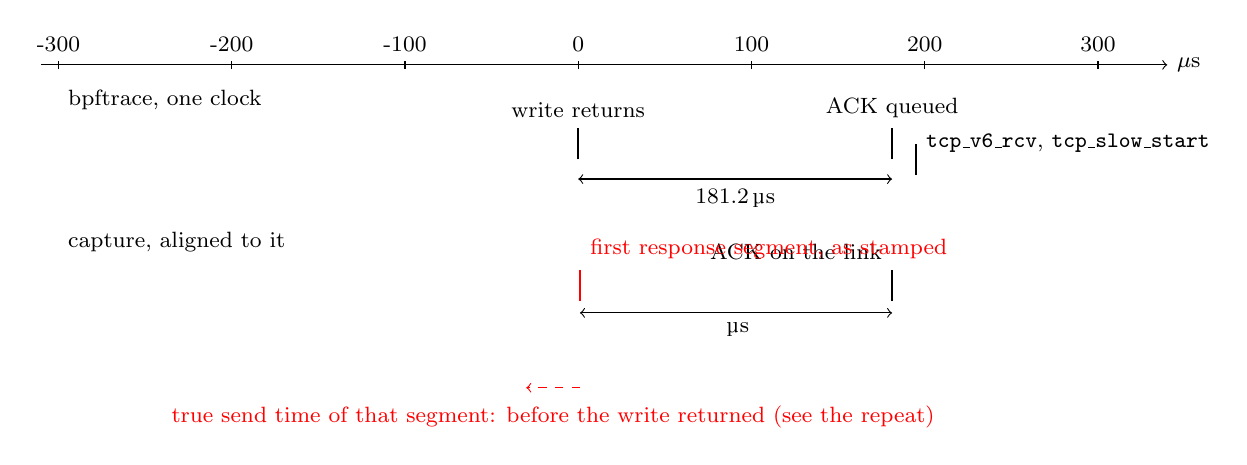
\begin{tikzpicture}[x=0.022cm, y=1cm, font=\footnotesize]
  \pgfmathsetmacro{\xe}{\HEnqMed}\pgfmathsetmacro{\xr}{\HEnqMed+\HWaitMed}\pgfmathsetmacro{\xs}{\ClkWriteAbs}
  \draw[->] (-310,2.2) -- (340,2.2) node[right] {$\mu$s};
  \foreach \t in {-300,-200,-100,0,100,200,300} {\draw (\t,2.15) -- (\t,2.25) node[above] {\t};}
  \node[anchor=west] at (-300,1.75) {bpftrace, one clock};
  \draw[thick] (0,1.0) -- (0,1.4) node[above] {write returns};
  \draw[thick] (\xe,1.0) -- (\xe,1.4) node[above] {ACK queued};
  \draw[thick] (\xr,0.8) -- (\xr,1.2) node[right] {\texttt{tcp\_v6\_rcv}, \texttt{tcp\_slow\_start}};
  \draw[<->] (0,0.75) -- node[below] {\HEnqMed\,\textmu s} (\xe,0.75);
  \node[anchor=west] at (-300,-0.05) {capture, aligned to it};
  \draw[thick] (\xe,-0.8) -- (\xe,-0.4) node[above left] {ACK on the link};
  \draw[thick,red] (\xs,-0.8) -- (\xs,-0.4) node[above right,red] {first response segment, as stamped};
  \draw[<->] (\xe,-0.95) -- node[below] {\HPcapMedAbsUs\,\textmu s} (\xs,-0.95);
  \draw[dashed,red,->] (\xs,-1.9) -- (-30,-1.9) node[midway,below=3pt,red] {true send time of that segment: before the write returned (see the repeat)};
\end{tikzpicture}
\caption{One late acknowledgment of the ticket on two clocks.}
\label{fig:timeline}
\end{figure}

\emph{When the acknowledgment counts.} The order of the ticket's acknowledgment and the response does not decide the window. Captures on the server's link (\RaceN\ resumed transactions, ten networks) show at least one ticket segment acknowledged before the response is written in \RaceBeforePct\% of them, including those where the window stayed at ten (read on the capture's clock, which orders a client packet and a server packet only to about a quarter of a millisecond, see Clocks; \RpKSixPct\% of \RpKSixN\ on one clock, Table~\ref{tab:clock}). What does separate the outcomes (a finding made afterwards) is the arrival of the ticket's last acknowledgment: the window exceeds ten segments when it comes more than \RaceThr\ms after the last request segment (\RaceRight\ of \RaceMlN\ ML-DSA transactions; exact 95\% interval \CiRaceLo--\CiRaceHi\%).

A request-size sweep with predictions committed beforehand confirmed the rule. Outside a borderline band (cells whose median lies within \RaceBand\ms of the threshold), \RaceTwoRight\ of \RaceTwoScored\ cells had the predicted class (95\% Wilson interval [90, 100]\%), and the rule classified \RaceTwoOosRight\ of \RaceTwoOosN\ transactions ([97, 99.5]\%). It gives the direction of the effect, not the size of the window. The controls with a small request are all right (\ECtlWrong\ of \ECtlN\ cells wrong). On this machine the rule barely depends on it (the table below: \ThrSLoR--\ThrSHiR\% of the transactions from 0.04 to 0.10\ms, \ThrSA\% at 0.02\ms), with the CPU clock fixed it carries over to a second x86 machine (see Repeat with every event on one clock), while its agreement with the kernel's state fails on Arm (Section~5 of the paper). The table gives the share of observations where ``the ACK arrives more than $T$ after the last request segment'' agrees with the outcome; $T=\RaceThr$\ms was chosen on the first run, so the table is post hoc.

\emph{What the kernel does.} A function trace of the server's kernel (criterion in the analysis script, committed before the run) covers \KerN\ acknowledgments of the ticket. Reno examines every one. It calls \texttt{tcp\_slow\_start} for none of the \KerBeforeN\ that arrive before the last request segment and for \KerAfterSS\% of the \KerAfterN\ that arrive after it. The rule classifies \KerRight\ of \KerN\ (\KerPct\%; exact interval \CiKerLo--\CiKerHi\%). The \KerWrong\ misses lie within \KerMissNear\ms of the threshold, about the resolution with which the two clocks are aligned.

A second run sidesteps the alignment problem by reading the sender's state at each acknowledgment (bpftrace probes on both functions; \StN\ acknowledgments, joined with the capture by port and acknowledgment number). \texttt{tcp\_\allowbreak slow\_\allowbreak start} is called iff the kernel's own test holds, i.e.\ \texttt{is\_\allowbreak cwnd\_\allowbreak limited} holds or \texttt{snd\_\allowbreak cwnd} is below twice \texttt{max\_\allowbreak packets\_\allowbreak out} (\StPOneRight\ of \StPOneN, as registered). Two other registered criteria failed (P2 and P3 of Table~\ref{tab:crit}). The threshold is a proxy, then, not the mechanism, and no constant of Linux TCP.

Looking at the data afterwards (post hoc), \StLateInflight\ of the \StLate\ acknowledgments that come more than \RaceThr\ms after the last request segment are processed with the response already in flight, where the test holds (median \texttt{packets\_out} \StAfterPk, against \StBeforePk\ for the others). Of the \StEarly\ acknowledgments up to \RaceThr\ms after it, \StEarlyLimited\ are limited, all of them ML-DSA-65, where \texttt{max\_packets\_out} reaches six and $10<2\times6$. A third group is more puzzling, with the reservation of Clocks: the capture shows \StDeferredN\ acknowledgments before the write but more than \RaceThr\ms after the last request segment, and \StDeferred\ of them are processed after the write. The window follows from the last acknowledgment of the ticket: the burst of the response equals the window after it (\StPTwoBRight\ of \StPTwoBN\ within one segment).

\emph{Why the acknowledgments are late, and the intervention.} Two explanations for the delay failed. The first asked whether socket ownership explains it (a third run, probes on the socket backlog; \BkN\ ticket acknowledgments). Only \BkDef\ were processed from the backlog, and both registered criteria failed (G1a and G1b of Table~\ref{tab:crit}). Afterwards we found that \texttt{tcp\_slow\_start} was called for all \PhAfterSS\ acknowledgments processed after the first write of the response returned, and for \PhBeforeSS\ of the \PhBefore\ processed before it (post hoc), most of them in softirq context. The second asked whether they wait in the softirq queue (a fourth run, probes on the queueing to the CPU backlog, on the receive path and on the softirq; \HN\ ticket acknowledgments), and it failed its registered criteria too. Only \HAOne\ of the \HALate\ late acknowledgments had been queued before the write returned (H1a of Table~\ref{tab:crit}), and the wait from queueing to processing was short (median \HWaitMed\,\textmu s, on the same CPU). Post hoc, they were queued a median \HEnqMed\,\textmu s after the write returned, while the capture puts them 0.07\ms before it; the two orderings differ by \ClkDiff\,\textmu s, the size of the uncertainty described under Clocks, and the order on the kernel's own clock is the one to trust: the acknowledgments reached the server's input queue after the write had returned, which is why that criterion failed.

An intervention at least settles the role of the ticket. When the server issues no ticket on resumed connections (predicted beforehand), the response burst is at most ten segments in all \NtkCells\ cells, including the \NtkEffect\ in which it exceeds ten with the ticket (exact sign test on those pairs $p=\SignNtkP$; with seven pairs no result can be smaller).

\begin{table}[h]
\caption{Robustness of the ticket-timing rule to its threshold $T$ (post hoc).}
\label{tab:thr}
\centering\small
\begin{tabular*}{\columnwidth}{@{\extracolsep{\fill}}p{0.30\columnwidth}rrrrrr@{}}
\toprule
$T$ (ms) & 0.02 & 0.04 & 0.049 & 0.06 & 0.08 & 0.10\\
\midrule
Burst $>10$, \RaceTwoOosN\ transactions (\%) & \ThrSA & \ThrSB & \ThrSC & \ThrSD & \ThrSE & \ThrSF\\
\texttt{tcp\_slow\_start} called, \StN\ ACKs (\%) & \ThrFA & \ThrFB & \ThrFC & \ThrFD & \ThrFE & \ThrFF\\
\bottomrule
\end{tabular*}
\end{table}

\section*{Repeat with every event on one clock}
The clock check led to a repeat of the traces on 21 November 2026 on the same machine (the X250) and, with the CPU clock fixed, on the Optiplex, with the procedure and the criteria K1 to K7 fixed beforehand (\texttt{results/wp6\_pred\_clock.md}). Before each trace \texttt{clock\_sync.py} reads the offset between the wall clock and the monotonic clock, the state of the kernel's clock, of NTP (switched off for the run) and of the CPU clock; after the trace it reads the offset again and refuses the file if it moved by more than 20\,\textmu s (\RpFiles\ of \RpFiles\ files passed). A new probe set, \texttt{ticket\_xmit.bt}, records on the \texttt{bpftrace} clock when each segment of the connection is handed to the device (XQ), when it leaves the queueing discipline, which is where \texttt{tcpdump} stamps it (XS), when a segment arrives (RX) and when the server's write returns, so that the true send time of the server's segments is read, not inferred. The repeat has the race design again (30 files) and the design of the softirq test again (6 files). It ran in two states of the CPU: first with the CPU clock as the system leaves it, then fixed (performance governor, no turbo) as in the first traces; the first repeat had left the clock to the system. Table~\ref{tab:clock} gives the outcomes.

\begin{table}[h]
\caption{Outcomes of the clock-safe repeat.}
\label{tab:clock}
\centering\footnotesize\setlength{\tabcolsep}{3pt}
\begin{tabular}{@{}p{0.24\textwidth}p{0.17\textwidth}p{0.17\textwidth}p{0.17\textwidth}p{0.14\textwidth}@{}}
\toprule
Criterion (fixed beforehand) & X250, CPU clock fixed & X250, clock as left & Optiplex, clock fixed & Outcome (fixed)\\
\midrule
K1 arrival stamps equal RX: at least 95\% within 20\,\textmu s, all within 50\,\textmu s & \RpKOnePct\%, largest \RpKOneMax\,\textmu s & \RuKOnePct\%, largest \RuKOneMax\,\textmu s & \RoKOnePct\%, largest \RoKOneMax\,\textmu s & not met on both\\
K2 capture stamp of a server segment equals XS: at least 95\% within 20\,\textmu s & \RpKTwoPct\% (median $\RpKTwoMed$\,\textmu s) & \RuKTwoPct\% (median $\RuKTwoMed$\,\textmu s) & \RoKTwoPct\% (median $\RoKTwoMed$\,\textmu s) & met on both\\
K3 delay that the device adds beyond RTT/2, per direction (reported) & \RpKThreeLo\ to \RpKThreeHi\,\textmu s, median \RpKThreeMed & \RuKThreeLo\ to \RuKThreeHi\,\textmu s, median \RuKThreeMed & \RoKThreeLo\ to \RoKThreeHi\,\textmu s, median \RoKThreeMed & reported\\
K4 first response segment queued before the write returns: at least 99\% & \RpKFourRight\ of \RpKFourN & \RuKFourRight\ of \RuKFourN & \RoKFourRight\ of \RoKFourN & met on both\\
K5 late acknowledgments reach the queue after that segment: at least 90\% & \RpKFiveRight\ of \RpKFiveN & \RuKFiveRight\ of \RuKFiveN & \RoKFiveRight\ of \RoKFiveN\ (too few to test) & met; Optiplex untested\\
K6 a ticket segment acknowledged before the write, overall and with a burst of ten or less, both at least 50\% (the sentence of Section~4 stays) & \RpKSixPct\% of \RpKSixN; \RpKSixSmallPct\% of \RpKSixSmallN & \RuKSixPct\% of \RuKSixN; \RuKSixSmallPct\% of \RuKSixSmallN & \RoKSixPct\% of \RoKSixN; \RoKSixSmallPct\% of \RoKSixSmallN & rule met on both: sentence stays\\
K7 rule of 0.049\ms on ML-DSA at MTU below 9\,000: transactions with a burst above ten, and the rule's accuracy (reported) & \RpKSevenPos\ of \RpKSevenN; \RpKSevenRight\ (\RpKSevenPct\%); best threshold \RpKSevenBestLo\ to \RpKSevenBestHi\ms & \RuKSevenPos\ of \RuKSevenN; \RuKSevenRight\ (\RuKSevenPct\%); best \RuKSevenBestLo\ms & \RoKSevenPos\ of \RoKSevenN; \RoKSevenRight\ (\RoKSevenPct\%); best \RoKSevenBestLo\ms & reported\\
\bottomrule
\end{tabular}
\end{table}

\emph{The clock.} The arrival stamps of the client's segments agree with RX to within $\RpKOneLo$ to $+\RpKOneHi$\,\textmu s for 90\% of the segments (5th to 95th percentile), with a tail to \RpKOneMax\,\textmu s (K1 and K2 of the three runs are in Table~\ref{tab:clock}). Once a constant is removed the stamps of the server's segments are within 20\,\textmu s of XS: \texttt{tcpdump} stamps a segment about \RpKTwoMed\,\textmu s from the tracepoint (negative: before it). With the CPU clock left to the system the stamps scatter more. The delay that the device adds beyond half the nominal RTT is about \RpKThreeMed\,\textmu s in each direction, and the analysis of the first traces moved the server's stamps back by the nominal half only; the 0.26\ms of the Clocks paragraph came from those traces and is of the same order.

\emph{The order.} On one clock the first segment of the response is queued before the write that sent it returns, in all \RpKFourN\ transactions, and the late acknowledgments reach the server's queue after that segment in all \RpKFiveN\ cases (K4 and K5 of Table~\ref{tab:clock}). The reading from the capture of the first traces, that the acknowledgment came before the response, was an effect of the stamps. The share of transactions with a ticket segment acknowledged before the response is written, \RaceBeforePct\% on the capture of the first run, is \RpKSixPct\% of \RpKSixN\ transactions with the correction (\RpKSixCapPct\% on the capture's own stamps for the same transactions), so the sentence of Section~4 stays with the new percentage.

\emph{The CPU clock.} The repeat with the clock left to the system did not reproduce the first traces. ECDSA-P256 had a burst of ten in every transaction of the first run (\BuFirstEcUp\ of \BuFirstEcN\ above ten), and in \BuPrEcUp\ of \BuPrEcN\ with the clock fixed (\BuPcEcUp\ of \BuPcEcN\ in a control with the instruments of the first run), but in \BuUrEcUp\ of \BuUrEcN\ with the clock left to the system (\BuUtEcUp\ of \BuUtEcN\ when repeated, \BuUcEcUp\ of \BuUcEcN\ with the instruments of the first run). The probes are therefore not the cause, and the control with the clock fixed reproduces the first traces (criterion T1, registered before it ran). Two settings of the clock were then separated on the X250, R2 only: with the performance governor and turbo on (3.2 GHz), ECDSA-P256 had a burst above ten in \BuIsolAEcUp\ of \BuIsolAEcN\ transactions, like the fixed clock, and the best threshold of the rule is \RaKSevenBestLo\ms; with the system's own governor (ondemand, the idle cores at 500 MHz in the record of \texttt{clock\_sync.py}) and turbo off, in \BuIsolBEcUp\ of \BuIsolBEcN, like the clock left to the system, and the best threshold is \RbKSevenBestLo\ms (K1 \RbKOnePct\%, K2 \RbKTwoPct\%, and \RbKSixPct\% of \RbKSixN\ transactions with a ticket segment acknowledged before the write). This is what we had predicted before the runs: the governor carries the difference and turbo does not. Nothing else was varied. The timing rule shows the same dependence: with the clock fixed the threshold of the first run, 0.049\ms, classifies \RpKSevenRight\ of \RpKSevenN\ transactions of the repeat (\RpKSevenPct\%) without being refitted, and the best threshold on these data is \RpKSevenBestLo\ to \RpKSevenBestHi\ms; with the clock left to the system the best threshold is \RuKSevenBestLo\ms. The threshold is thus a property of the state of the machine, not of Linux TCP.

Figure~\ref{fig:k7} shows the transactions behind these numbers: with the clock fixed the two groups are separated at 0.049\ms (the vertical line), with turbo off or the clock as left, and on the Arm machine, the transactions with a burst above ten lie further right and the groups overlap.

\begin{figure}[h]
\centering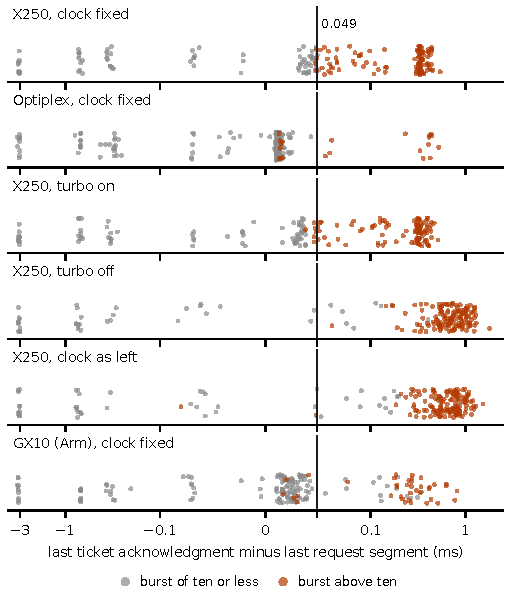
\includegraphics[width=0.62\textwidth]{fig_k7_points}
\caption{Each ML-DSA transaction at MTU below 9\,000, by the gap of its last ticket acknowledgment to the last request segment.}
\label{fig:k7}
\end{figure}

\emph{Run to run.} The same repeat on the X250 once more, with the CPU clock fixed, agrees with the first: K2 and K4 are met (\RqKTwoPct\%, \RqKFourRight\ of \RqKFourN), K5 is met (\RqKFiveRight\ of \RqKFiveN), K1 is not met again (\RqKOnePct\%), \RqKSixPct\% of \RqKSixN\ transactions have a ticket segment acknowledged before the write (against \RpKSixPct\%), and the rule of 0.049\ms classifies \RqKSevenRight\ of \RqKSevenN\ ML-DSA transactions (\RqKSevenPct\%, against \RpKSevenPct\%) with a best threshold of \RqKSevenBestLo\ms. The agreement criteria registered beforehand (within 5 points on the share and on the accuracy, within 0.02\ms on the threshold) are met, so the two figures are a range of two runs rather than one number.

\emph{A second machine.} The same repeat on the Optiplex (i7-8700, Linux 7.0.0-42, the CPU clock fixed) gives the same picture of the clock (Table~\ref{tab:clock}), with one difference of degree: the device adds more delay on this machine, about \RoKThreeMed\,\textmu s beyond RTT/2 at the longer RTTs against \RpKThreeMed\,\textmu s on the X250 (K3). The share of transactions with a ticket segment acknowledged before the write is \RoKSixPct\% (K6), so the sentence of Section~4 holds on both machines. The ticket enlarges the server's window much more rarely on the Optiplex: of the \RoKSevenN\ ML-DSA transactions at MTU below 9\,000 the burst exceeds ten in \RoKSevenPos\ (\RpKSevenPos\ on the X250), so the softirq design gave too few late acknowledgments for K5 (\RoKFiveN). The rule of 0.049\ms still separates them, \RoKSevenRight\ of \RoKSevenN\ without refitting (\RoKSevenPct\%; the trivial answer, a burst of ten in every transaction, gets \the\numexpr\RoKSevenN-\RoKSevenPos\relax), and the best threshold is \RoKSevenBestLo\ms. We had written beforehand that the Optiplex's best threshold would differ from the X250's by more than 0.02\ms; it differs by \RoKSevenDiff\ms, so that prediction failed, and the threshold carried over to this second x86 machine once the CPU clock was fixed.

\emph{The Arm machine.} The same repeat on the GX10 (Cortex-A725 and X925, Linux 7.0.0-1025, client on CPU~0 and server on CPU~1 as in the earlier Arm traces; the CPU clock read as fixed: governor performance, no boost) had five predictions registered beforehand (D1 to D5), and three were met. K4 holds (\RgKFourRight\ of \RgKFourN) and so does K5 (\RgKFiveRight\ of \RgKFiveN), the ticket enlarges the server's window rarely (a burst above ten in \RgKSevenPos\ of \RgKSevenN\ ML-DSA transactions at MTU below 9\,000, at most a quarter predicted), and \RgKSixPct\% of \RgKSixN\ transactions have a ticket segment acknowledged before the write (\RgKSixSmallPct\% of \RgKSixSmallN\ with a burst of ten or less). Two were not met. K2 reached \RgKTwoPct\% within 20\,\textmu s (95\% required), and the rule of 0.049\ms classifies \RgKSevenRight\ of \RgKSevenN\ transactions (\RgKSevenPct\%; 90\% required; the trivial answer gets \the\numexpr\RgKSevenN-\RgKSevenPos\relax) with a best threshold of \RgKSevenBestLo\ms, against 0.047 to 0.048\ms on the X250 and 0.057\ms on the Optiplex. K1 is not met either (\RgKOnePct\% within 20\,\textmu s, largest \RgKOneMax\,\textmu s), and the device adds \RgKThreeLo\ to \RgKThreeHi\,\textmu s beyond RTT/2. With every event on one clock the threshold therefore does not carry over to Arm, as the registered reading of D4 says; the sentence of Section~4 holds (K6), and the state test, which this repeat does not redo, stays as registered.

\section*{The same tests on other machines}
On 21 November 2026 the random design of the paper (row 20 of Table~1 of the paper) was measured on three more runs, with criteria fixed beforehand: on the Arm machine and on a second x86 machine (A1 to A4, the first X250 run as reference) and again on the X250 (V1 to V3). The ticket tests on new cells and with delayed acknowledgments (rows 16 and 18) were measured on the same two machines (K1 to K4 and D1 to D5). Table~\ref{tab:cells} lists the cells that the model got wrong in at least one of the four runs of the random design; a cell is wrong when the model is off by more than half the RTT, and the measured excess is the median of the resumed transactions on the shaped link minus the median on the unshaped base.

\begin{table}[h]
\caption{Cells the model got wrong in at least one run (measured excess in ms; bold: wrong).}
\label{tab:cells}
\centering\footnotesize\setlength{\tabcolsep}{4pt}
\begin{tabular}{@{}rllrrrrrrr@{}}
\toprule
Cell & Suite & RTT & Request / response (B) & Model & X250 run 1 & X250 run 2 & GX10 & Optiplex\\
\midrule
\GnineCellRows
\bottomrule
\end{tabular}
\end{table}

\begin{figure}[h]
\centering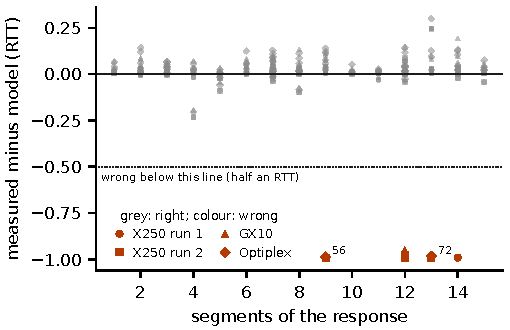
\includegraphics[width=0.62\textwidth]{fig_cells_map}
\caption{Error of the model in round trips against the segments of the response, one mark per cell and run.}
\label{fig:cellsmap}
\end{figure}

The model is wrong on \GnineCellsWrongXOne\ cells of the first X250 run, \GnineCellsWrongXTwo\ of its repeat, \GnineCellsWrongGx\ on the Arm machine and \GnineCellsWrongOp\ on the Optiplex, and \GnineCellsEvery\ cells (56 and 72) are wrong on every run. Every wrong cell is a round trip faster than the model says (Figure~\ref{fig:cellsmap}: all lie at $-1$ RTT, in responses of \GnineRespLo\ to \GnineRespHi\ segments). The other cells that fail do so on some machines only: criterion A2 (at least four of the five cells wrong on the first X250 run are wrong on the second machine) is met on the Arm machine and not met on the Optiplex, and V1 (the same on the X250 again) is met. We read this as the registered rule says: the region where the model fails depends in part on the machine, a statement about the server's window, not a failure of the model to follow the ticket. The ticket tests of rows 16 and 18 are met on both machines (\GtwelveRepMet\ of \GtwelveRepK\ criteria).

\section*{A second random draw}
After the predictions of the paper were fixed we drew 100 further cells at random from the design space of the random draw of the paper (row 20 of Table~1 of the paper; another seed, no cell reused) and measured them on the X250 and on the Arm machine, with the predictions of the model written down before any measurement (\texttt{results/g22\_round2\_predictions.md}). The model was wrong by more than half an RTT on \GttXRWrong\ of the \GttXRN\ cells on the X250 (mean absolute error \GttXRMae\,ms; \GttXRTwo\ cells within 2\,ms) and on \GttARWrong\ on the Arm machine (\GttARMae\,ms; \GttARTwo\ cells within 2\,ms, the rest a constant offset of about 3\,ms of that machine). With the first draw of the paper (Table~\ref{tab:cells}) the model was wrong on \GnineCellsWrongXOne\ and \GttXRWrong\ of 100 cells on the X250 and on \GnineCellsWrongGx\ and \GttARWrong\ on the Arm machine. We measured \GttXFN\ further cells, chosen and not random: those on which an alternative model of the ticket's acknowledgments (not part of this paper) predicted a faster response than the model of the paper. The model was wrong on \GttXFWrong\ of them on the X250 and on \GttAFWrong\ on the Arm machine, as expected in the region where the server's window after the ticket is larger than ten, which the model does not predict. All \GttDirSlow\ wrong cell-runs of this draw (of \GttDirRuns) are too slow and none is too fast; the largest underestimate is \GttDirMaxX\,ms on the X250 and \GttDirMaxA\,ms on the Arm machine. The criteria registered for this draw concerned the alternative model, not rule~(1), so the numbers for the model of the paper are reported, not tested; the regions where the model fails depend on the machine, as in the first draw. We also repeated the measurement of the X250 once, declared before it as a run to find the noise floor: the same cells, the same predictions. The model was then wrong on \GttXRunTwoWrong\ of the 100 cells (mean absolute error \GttXRunTwoMae\,ms) instead of \GttXRWrong, and the measured excess of \GttXNoise\ of the 130 cells differs between the two runs by more than half an RTT. The count of wrong cells of a run of 100 therefore has a noise of a few cells; no error in the wrong direction (too fast) appeared in the repeat either.

\section*{Direction of the errors}
With Reno or Cubic the model of the paper is wrong by more than half an RTT in \OsSlow\ of \OsRuns\ cell-runs, and every one of these \OsSlow\ is too slow: the measured excess is below the prediction. In no cell-run is it too fast by that margin. Table~\ref{tab:dir} counts the cell-runs of the tests that have a per-cell prediction of the model (client window, ticket timing, new cells, delayed acknowledgments, a real link, background load and the random draw, on three machines). The same cell appears in several runs (three OpenSSL releases, three machines), so the \OsRuns\ cell-runs are \OsCells\ cells, each counted once per test. The reason is that the model gives the server a window of ten after the ticket, the least it can have: the ticket can only enlarge it. Not covered are loss, MTU 9\,000, Go and full handshakes, and BBR, whose window is not rule~(1): under BBR two cells are too fast, the two ML-DSA-87 cells that Section~6 reports between the BBR and the Reno prediction. With delayed acknowledgments the model is too fast by up to \OsMaxDelack\,ms, the delayed-ACK timer that it leaves out and less than half an RTT; elsewhere the largest underestimate is \OsMaxElse\,ms.

\begin{table}[h]
\caption{Cell-runs by direction of the error, with errors of more than half an RTT counted.}
\label{tab:dir}
\centering\footnotesize\setlength{\tabcolsep}{4pt}
\begin{tabular}{@{}lrrrr@{}}
\toprule
Test & Runs & Cell-runs & Too fast & Too slow\\
\midrule
\OsRows
\bottomrule
\end{tabular}
\end{table}

\section*{Details that the paper summarises}
This section gives, for sentences of the paper that can only be short, the data behind them, in the order of the paper.

\emph{The 13 configurations of stage A (Section~3).} Table~\ref{tab:stagea} lists them. Every configuration was read at the same 20 flight sizes ($n_1=1\dots16,20,24,31,40$) with 20 connections each; a size ``matches'' when the median window afterwards equals rule~(1) with the initial window of the configuration. Twelve configurations match at all 20 sizes. At MTU 9\,000 only 7 of 20 match, for the reason given in Section~3 of the paper: the receive window limits the sender, \texttt{is\_cwnd\_limited} stays false and the window does not grow.

\begin{table}[h]
\caption{Flight sizes at which the median window equals rule~(1), by configuration of stage A.}
\label{tab:stagea}
\centering\footnotesize\setlength{\tabcolsep}{4pt}
\begin{tabular}{@{}lrrrr@{}}
\toprule
Configuration (one factor changed from the base) & $w_0$ & Sizes & Connections & Sizes matching\\
\midrule
\StageARows
\bottomrule
\end{tabular}
\end{table}

\emph{The ticket-size error (Section~6).} The one discriminating cell that the early-ticket model got wrong in the random draw is an ECDSA-P256 cell with a small request, where the joined-ticket model was right. The ticket of the model is \TktDiffLo\ to \TktDiffHi\ bytes larger than the one on the wire (\TktModelEc\ against \TktWireEc\ bytes for ECDSA-P256), which at the MSS of that cell turns one segment into two and pushes ticket and response past the window of ten. With the measured size that prediction changes from \TktCellOld\ to \TktCellNew\,ms, and no other prediction of the \GnineN\ cells changes by more than 1\,ms. We found the error afterwards and tested it with predictions fixed first (row 26): the cell measured again with $n=200$ gave \GnineBRepeat\,ms, as before; the model with the measured ticket size was right on all six cells of that family (responses of 9\,500 to 12\,400\,B), the earlier model on none of the \GnineBDisc\ cells where the two differ, and the step from three to four round trips lies between \GnineBLo\ and \GnineBHi\,B.

\emph{Cells off by a few milliseconds (Section~6).} In the random draw the model is right to within half an RTT on 95 of the 100 cells and to within 2\,ms on 85. The ten cells in between are all at 10\,Mbit/s and are off by \GnineOffLo\ to \GnineOffHi\,ms (Table~\ref{tab:offcells}; positive: the model is slower than the measurement). The errors have both signs and are far below an RTT; we did not look for their cause. Hence the section on the direction of the errors counts only errors of more than half an RTT: at the level of milliseconds the model is not one-sided.

\begin{table}[h]
\caption{The ten cells of the random draw that are off by more than 2\,ms but by less than half an RTT (first X250 run).}
\label{tab:offcells}
\centering\footnotesize\setlength{\tabcolsep}{4pt}
\begin{tabular}{@{}rlrrrrr@{}}
\toprule
Cell & Suite & RTT (ms) & Rate (Mbit/s) & MTU & Request / response (B) & Error (ms)\\
\midrule
\OffRows
\bottomrule
\end{tabular}
\end{table}

\emph{Background load (Section~6).} The four levels of row 24 were: L0 no load (the control); L1 cross traffic on the link (UDP at 40\,Mbit/s and ten TCP connections of 2\,Mbit/s each; \GseventeenUdp\ and \GseventeenTcp\,Mbit/s were achieved, about 58\,\% of the 100\,Mbit/s link); L2 a busy loop on every CPU, including those of the client and server probes; L3 both. The \GseventeenCells\ cells are the client-window and ticket-timing cells of row 18 ($n=30$, predictions unchanged). At every level the model was wrong on at most \GseventeenWrongMax\ of the \GseventeenCells\ cells and the joined-ticket model on at least \GseventeenJoinedMin\ of the \GseventeenDisc\ discriminating cells; the load moved the excess of a cell by at most \GseventeenShiftMax\,ms against no load. The traffic is one fixed mix on one bottleneck and the busy loop stands for a loaded host: neither stands for production traffic.

\emph{Tails (Section~6).} Table~\ref{tab:tails} gives the six cells measured with $n=1\,000$ transactions each (row 22). Each has one narrow peak: the maximum is at most 2.5\,ms above the median, and no transaction exceeds its median by 20\,ms, so the tail hides no second step of one round trip in these cells. Six cells are a small sample, not a survey of the design space.

\begin{table}[h]
\caption{Latency of the six cells with $n=1\,000$ (ms; the last column is the share of transactions above the median by more than 20\,ms, in \%).}
\label{tab:tails}
\centering\footnotesize\setlength{\tabcolsep}{4pt}
\begin{tabular}{@{}llrrrrrr@{}}
\toprule
Suite & Request / response (B) & $n$ & Median & P99 & P99.9 & Max & Above 20\,ms\\
\midrule
\TailRows
\bottomrule
\end{tabular}
\end{table}

\emph{Runs that preceded the reported ones.} The real-link test (row 25) began with a smoke run of $n=3$; its plain-TCP part was complete and gave the same result, and it is not used. The first run of the test on Go (row 14) lacked the ECDSA-P256 set; that set was measured again on its own, on the same machine, and the two runs are merged for the criteria H1 to H5, with the predictions and the criteria unchanged. The traces of the ticket's acknowledgments were repeated with every event on one clock after the first traces had been read (Section ``Repeat with every event on one clock''); the first traces are kept and reported.

\section*{What remains open}
\emph{Established.} (i) The ticket matters: without it the burst is at most ten segments in every cell (the intervention). (ii) The window after it follows from the last acknowledgment of the ticket: the burst of the response equals the window left after it (\StPTwoBRight\ of \StPTwoBN\ within one segment), and \texttt{tcp\_slow\_start} runs exactly when the kernel's own test holds (\StPOneRight\ of \StPOneN). (iii) That test holds when the acknowledgment is processed with the response already in flight (post hoc: \StLateInflight\ of \StLate). (iv) The late acknowledgments, those processed after the first write of the response has returned, reach the server's input queue after that return (a median \HEnqMed\,\textmu s on the \texttt{bpftrace} clock) and are processed within \HWaitMed\,\textmu s, on the same CPU.

\emph{Refuted.} (i) That a larger client window explains the model's error on the request flight (the loosened rule, Table~1 of the paper). (ii) That the ticket is written with the response (the joined-ticket model). (iii) That socket ownership or the softirq queue delays the acknowledgments (criteria G1a, G1b, H1a, H1b). (iv) That the acknowledgment precedes the response: the reading from the capture's clock was an effect of the stamps. (v) That the threshold of 0.049\ms holds on every machine and CPU clock (it does not on Arm, nor with the clock left to the system).

\emph{Not established.} Why those acknowledgments reach the server's queue some \HEnqMed\,\textmu s after the write. Two candidates were tested and failed (socket ownership, the softirq queue); both would have acted inside the server's host after the queue, and the data put the delay before it, on the path from the client's \texttt{netem} through the virtual link. Whether this happens only in the emulated link is not settled: the ticket cells give the predicted windows on a cable between two machines (row 25 of Table~1 of the paper), which speaks against an artefact of the emulation but was not traced there. The timing rule of 0.049\ms is a proxy for this ordering at the server, found on the first run; it holds on the same machine with the CPU clock fixed and not with the clock left to the system, it carried over to a second x86 machine with the clock fixed, but not to Arm with every event on one clock, where its agreement with the kernel's state had also failed; it is not a constant of Linux TCP. The share of transactions with a ticket segment acknowledged before the write is \RaceBeforePct\% on the capture of the first run and \RpKSixPct\% with every event on one clock (Table~\ref{tab:clock}). The repeat with every event on one clock (previous section) removed the doubt about the order: on the host's own clock the acknowledgments that count reach the queue after the response has been queued, and the cause of that is still open.

\emph{Next measurements.} (i) The acknowledgment at the NIC, in the driver and in the receive path of the server, to place the delay of \HEnqMed\,\textmu s. (ii) The same ticket cells on a physical path whose delay is not made by \texttt{netem}, with the probes of this supplement. (iii) The server's window after the ticket as a function of the order in which its acknowledgments are processed, per machine, which the paper's rule (1) does not predict. (iv) Tails on more cells near the boundary of the window and with several concurrent connections. None of these is in the paper.

\section*{What each part of the model adds}
Table~\ref{tab:ablation} gives the mean absolute error (MAE, in ms) of each model and the number of cells it gets wrong by a round trip.

\begin{table}[h]
\caption{What each part of the model adds.}
\label{tab:ablation}
\centering\footnotesize\setlength{\tabcolsep}{4pt}
\begin{tabular}{@{}lrrrr@{}}
\toprule
 & \multicolumn{2}{c}{\AblFixedN\ resumed} & \multicolumn{2}{c}{\AblCFixedN\ client window}\\
Model & MAE & wrong & MAE & wrong\\
\midrule
Window fixed at $w_0$ & \AblFixedMae & \AblFixedOff & \AblCFixedMae & \AblCFixedOff\\
Textbook slow start & \AblSlowMae & \AblSlowOff & \AblCSlowMae & \AblCSlowOff\\
+ Linux validation, rule (1) & \AblLinuxMae & \AblLinuxOff & \AblCLinuxMae & \AblCLinuxOff\\
+ OpenSSL write pattern, ticket joined & \AblJoinedMae & \AblJoinedOff & --- & ---\\
+ ticket written on the Finished & \AblEarlyMae & \AblEarlyOff & --- & ---\\
\bottomrule
\end{tabular}
\end{table}

\section*{Where each number comes from}
Table~\ref{tab:repro} lists the script and the output behind each number. Scripts are in \texttt{Measurements/testbed/}, outputs in \texttt{Measurements/testbed/results/}; \texttt{make\_assets\_short.py} (in \texttt{paper2\_short/Latex/}) reads the outputs and writes every number of the paper and of this supplement to \texttt{numbers\_short.tex}. The raw traces are on Zenodo (the ticket tests: doi:\allowbreak10.5281/\allowbreak zenodo.\allowbreak24384873; the clock-safe repeat: doi:\allowbreak10.5281/\allowbreak zenodo.\allowbreak24419058); \texttt{tools/raw\_traces.sh verify} reruns the analyses on them and compares the outputs with the archive.

\begin{table}[h]
\caption{Scripts and outputs.}
\label{tab:repro}
\centering\footnotesize\setlength{\tabcolsep}{4pt}
\begin{tabular}{@{}p{0.40\textwidth}p{0.25\textwidth}p{0.28\textwidth}@{}}
\toprule
Number & Script & Output\\
\midrule
Captures: \RaceN\ transactions, \RaceBeforePct\%, \RaceRight\ of \RaceMlN & \texttt{analyze\_ticket\_race.py} & \texttt{ticket\_race.csv}, \texttt{wp6\_analysis\_race.txt}\\
Sweep: \RaceTwoRight\ of \RaceTwoScored, \RaceTwoOosRight\ of \RaceTwoOosN & \texttt{analyze\_race2.py} & \texttt{wp6\_analysis\_race2.txt}\\
Threshold table & \texttt{threshold\_sweep.py} & \texttt{wp6\_analysis\_threshold.txt}\\
Function trace: \KerRight\ of \KerN & \texttt{analyze\_ftrace.py} & \texttt{wp6\_analysis\_kernel.txt}\\
State trace: \StN, P1--P3 & \texttt{analyze\_state.py} & \texttt{wp6\_analysis\_state.txt}, \texttt{ticket\_state.csv}\\
Backlog: \BkN & \texttt{analyze\_backlog.py}, \texttt{analyze\_backlog\_posthoc.py} & \texttt{wp6\_analysis\_backlog.txt}, \texttt{wp6\_analysis\_backlog\_posthoc.txt}\\
Softirq: \HN, \HALate, \HEnqMed\,\textmu s & \texttt{analyze\_softirq.py}, \texttt{analyze\_softirq\_posthoc.py} & \texttt{wp6\_analysis\_softirq.txt}, \texttt{wp6\_analysis\_softirq\_posthoc.txt}\\
No ticket: \NtkCells\ cells, $p=\SignNtkP$ & \texttt{analyze\_notkt.py} & \texttt{wp6\_analysis\_notkt.txt}\\
Clocks: \ClkN\ acknowledgments & \texttt{analyze\_clock\_check.py} & \texttt{wp6\_clock\_check.txt}\\
Other machines: A1--A4, V1--V3, K1--K4, D1--D5 & \texttt{analyze\_\allowbreak g19\_\allowbreak arm.py}, \texttt{analyze\_\allowbreak g12.py}, \texttt{analyze\_\allowbreak g14.py} & \texttt{g19\_\allowbreak *\_\allowbreak analysis.txt}, \texttt{g12\_\allowbreak *\_\allowbreak analysis.txt}, \texttt{g14\_\allowbreak *\_\allowbreak analysis\_\allowbreak delack.txt}\\
Clock-safe repeat (Table~\ref{tab:clock}) & \texttt{clock\_sync.py}, \texttt{ticket\_\allowbreak xmit.bt}, \texttt{analyze\_\allowbreak clock\_\allowbreak repeat.py}, \texttt{compare\_\allowbreak race\_\allowbreak bursts.py} & \texttt{wp6\_clock\_\allowbreak repeat\_\allowbreak tuned\_\allowbreak analysis.txt}, \texttt{wp6\_clock\_\allowbreak repeat\_\allowbreak analysis.txt}, \texttt{wp6\_clock\_\allowbreak repeat\_\allowbreak bursts.txt}, \texttt{wp6\_\allowbreak clock\_\allowbreak repeat\_\allowbreak gx10\_\allowbreak analysis.txt}, \texttt{wp6\_\allowbreak k7\_\allowbreak points\_\allowbreak *.csv} (Figure~\ref{fig:k7})\\
Cells of the random design (Figure~\ref{fig:cellsmap}) & \texttt{make\_\allowbreak assets\_\allowbreak short.py} & \texttt{g19\_\allowbreak *\_\allowbreak cells.txt}\\
Second random draw (G22): \GttXRN\ random cells per machine & \texttt{g22\_\allowbreak predict.py}, \texttt{analyze\_\allowbreak g22.py} & \texttt{g22\_\allowbreak *\_\allowbreak analysis.txt}, \texttt{g22\_\allowbreak predictions.csv}\\
Direction of the errors (Table~\ref{tab:dir}) & \texttt{one\_\allowbreak sided\_\allowbreak errors.py} & \texttt{one\_\allowbreak sided\_\allowbreak errors.txt}\\
Segment counts of Dubetskyy and Cano (Section~4 of the paper) & \texttt{analyze\_\allowbreak dubetskyy\_\allowbreak segments.py} & \texttt{dubetskyy\_\allowbreak segments\_\allowbreak 20261116.txt}\\
OpenSSL ticket code across releases (Section~6 of the paper) & \texttt{audit\_\allowbreak ossl\_\allowbreak ticket\_\allowbreak path.py} & \texttt{ossl\_\allowbreak ticket\_\allowbreak path\_\allowbreak audit.txt}\\
Model components (last table) & \texttt{analyze\_l1\_model\_comparison.py} & \texttt{l1\_model\_comparison.csv}, \texttt{.txt}\\
\bottomrule
\end{tabular}
\end{table}
\end{document}
